\documentclass[12pt]{report}

\usepackage{cmap}
\usepackage[T1,T2A]{fontenc}
\usepackage[utf8]{inputenc}
\usepackage[english, russian]{babel}
\usepackage{amssymb}
\usepackage{amsmath}
\usepackage{amsthm}
\usepackage{dsfont}
\usepackage{bm}
\usepackage{diagbox}
\usepackage[left=20mm,right=10mm,top=20mm,bottom=20mm,bindingoffset=2mm]{geometry}
\usepackage{indentfirst}
\usepackage[utf8]{inputenc}
\usepackage{float}
\usepackage[hidelinks]{hyperref}
\usepackage{graphicx}
\usepackage{xcolor}
\usepackage{listings}
\usepackage{minted}

\DeclareMathOperator{\N}{\mathbb{N}}
\DeclareMathOperator{\R}{\mathbb{R}}
\DeclareMathOperator{\Z}{\mathbb{Z}}
\DeclareMathOperator{\CC}{\mathbb{C}}
\DeclareMathOperator{\PP}{\mathrm{P}}
\DeclareMathOperator{\Expec}{\mathrm{E}}
\DeclareMathOperator{\Var}{\mathrm{Var}}
\DeclareMathOperator{\Cov}{\mathrm{Cov}}
\DeclareMathOperator{\asConv}{\xrightarrow{a.s.}}
\DeclareMathOperator{\LpConv}{\xrightarrow{Lp}}
\DeclareMathOperator{\pConv}{\xrightarrow{p}}
\DeclareMathOperator{\dConv}{\xrightarrow{d}}

\hypersetup{
	colorlinks=true,
	linkcolor=blue,
	citecolor=blue,
	urlcolor=blue
}

\lstset{language=Python, extendedchars=\true}

\lstdefinestyle{pythonstyle}{
	language=Python,
	backgroundcolor=\color{lightgray},
	commentstyle=\color{green},
	keywordstyle=\color{blue},
	stringstyle=\color{red},
	basicstyle=\ttfamily,
	frame=single,
	breaklines=true
}

\begin{document}
	
	\begin{titlepage}
		\begin{center}
			\large{Федеральное государственное автономное образовательное учреждение высшего образования <<Национальный исследовательский университет ИТМО>>}
		\end{center}
		
		\vspace{15em}
		
		\begin{center}
			\huge{\textbf{Курсовая работа}} \\
			\large{По дисциплине <<Проектирование Пользовательских Интерфейсов>>} \\
			\large{Задание №3} \\
		\end{center}
		
		\vspace{2em}
		
		\begin{flushright}
			\textit{\large{Выполнили:}} \\
			\large{Студент группы P3306} \\
			\large{Михайлов Дмитрий} \\
			\large{Андреевич} \\
			\large{Студент группы P3317} \\
			\large{Мищенко Роман} \\
			\large{Андреевич} \\
			\textit{\large{Преподаватель:}} \\
			\large{Балканский Андрей} \\
			\large{Александрович}
		\end{flushright}
		
		\vspace{2cm}
		
		\begin{figure}[h]
			\centering
			
\includegraphics[width=0.5\linewidth]{image.png}
		\end{figure}
		
		\begin{center}
			Санкт-Петербург \\
			2025 год
		\end{center}
	\end{titlepage}
	
	\tableofcontents
	\newpage
	
	\addcontentsline{toc}{section}{Задание}
	\section*{Задание}
	Разработать информационную архитектуру (структуру, информационные элементы, названия разделов). Не нужно указывать, где какая кнопка/картинка(это будет видно после выполнения 4 лабораторной), только информационная структура из разделов и сущностей.
	\begin{enumerate}
		\item Декомпозиция - выделите информационные сущности(страницы, товары, пользователи и т.д.) и опишите их свойства(какую информацию содержит в себе сущность: id, название, описание, изображение, размер и т.д.) \\
		
		\item Рассмотрите, как взаимодействуют между собой сущности, являются они вложенными(как каталог->категория->товар) или равными, составьте структуру информационной системы. Для навигации по продукту старайтесь использовать до 4 основных разделов (максимум 7), а остальные делать вложенными в один из основных. \\
		
		\item Проверьте, понятные ли названия у компонентов вашей системы. Для этого обратитесь к человеку из вашей целевой аудитории, кратко опишите ему идею вашего продукта, и попросите его описать, какая информация находиться под тем или иным элементом системы. Следите за длиной названия(если более 3 слов, то возможно стоит разнести этот компонент на два) \\
		
		\item Схематизация - составьте схему информационной архитектуры в формате текста/блок-схемы \\
		
		\item Загрузите схему информационной системы на яндекс-диск. \\
	\end{enumerate}
	\newpage
	
	\addcontentsline{toc}{section}{ER-model}
	\section*{ER-model}
	
	\begin{figure}[h]
		\centering
		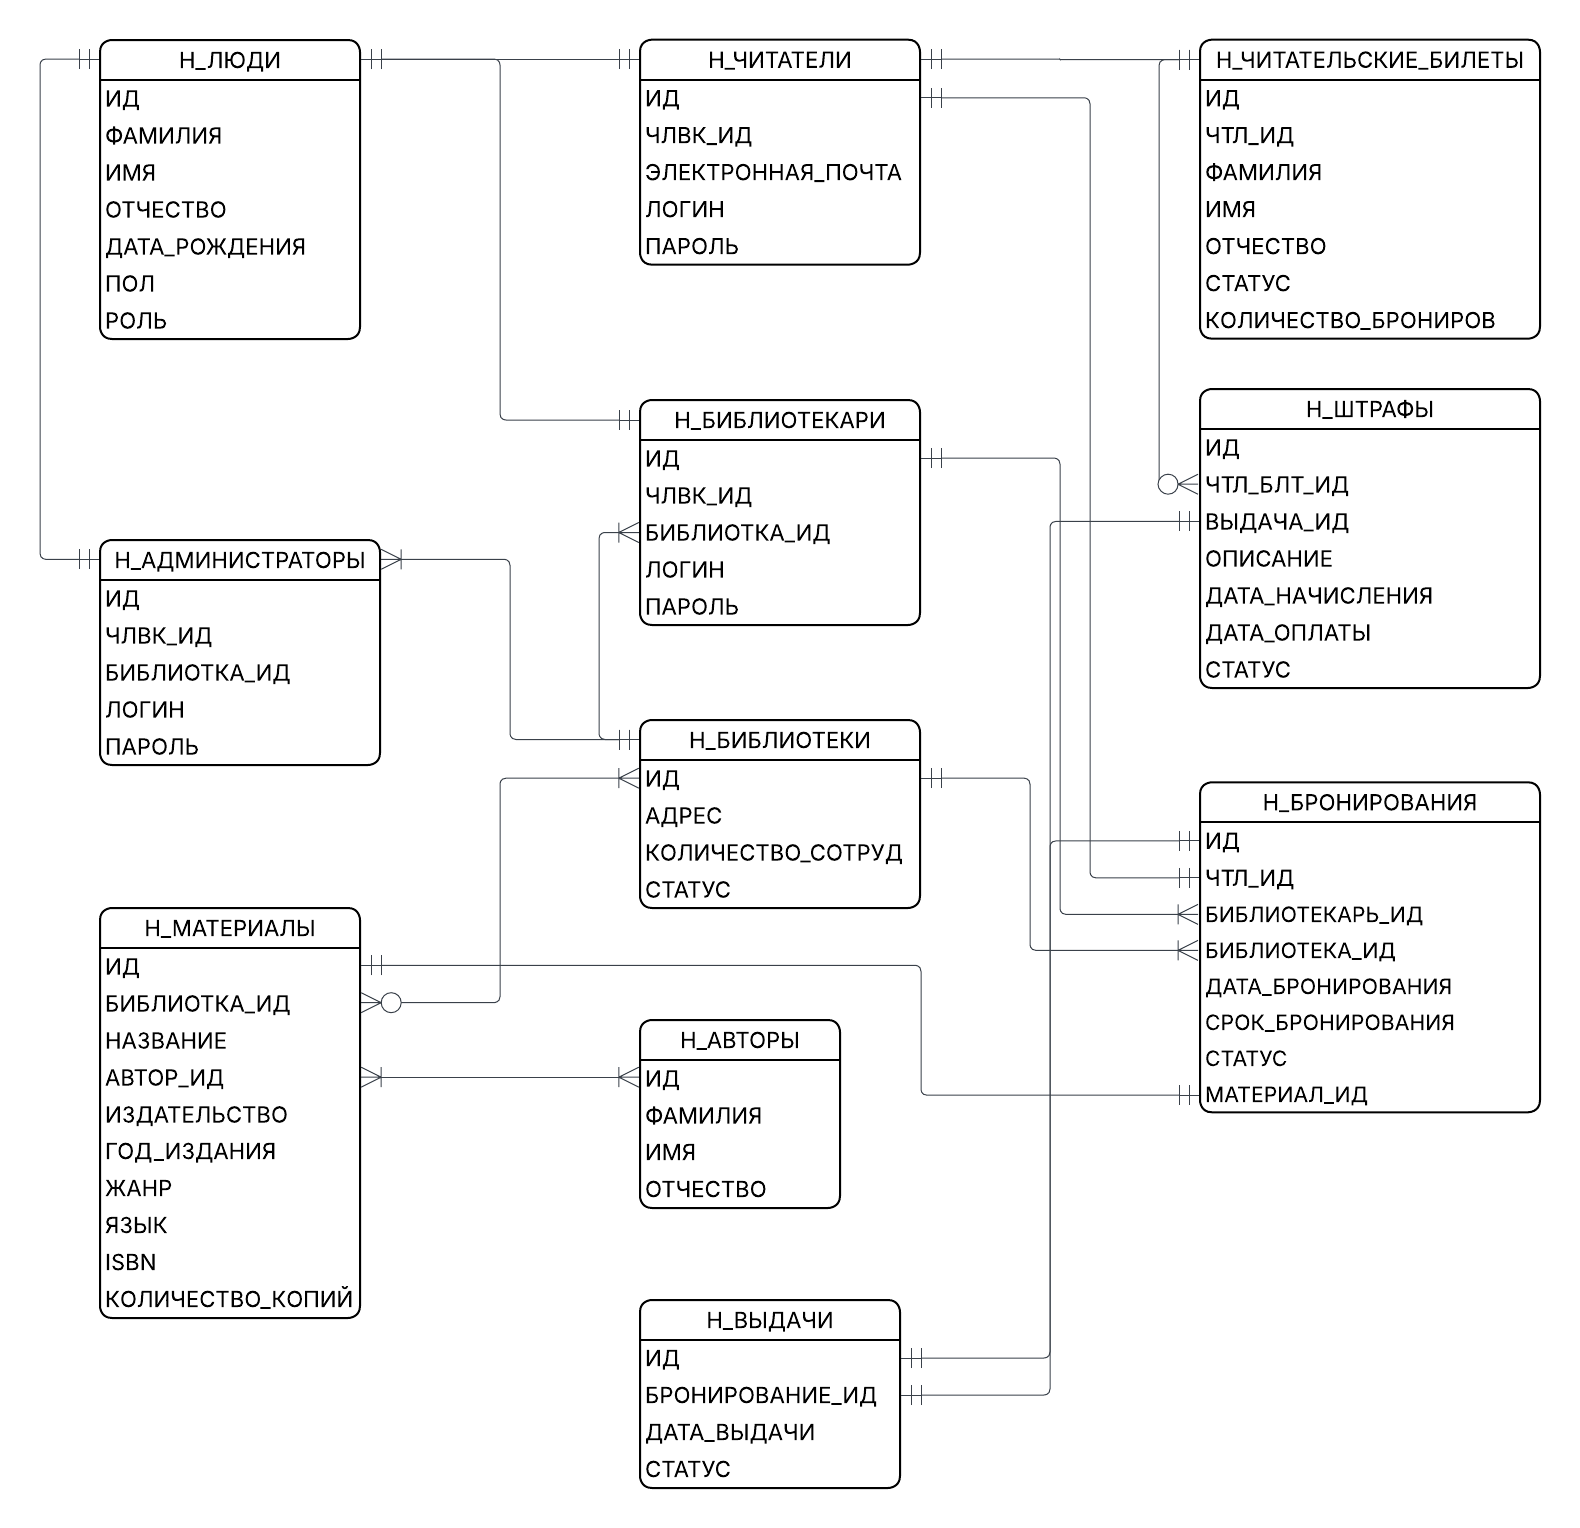
\includegraphics[width=0.8\textwidth]{ER-model.png}
		\caption{ER-модель на основе описаний предметной области и прецедентов из предыдущего этапа.}
		\label{fig:ER-model}
	\end{figure}
	\newpage
	
	\addcontentsline{toc}{section}{Информационная архитектура}
	\section*{Информационная архитектура}
	
	
\end{document}
